% !TEX TS-program = pdflatex
% !TEX encoding = UTF-8 Unicode
% arara: pdflatex: { synctex: true }
\pdfminorversion=7
% \PassOptionsToPackage{rgb,svgnames,dvipsnames,x11names}{xcolor}
\documentclass[tikz,border=10pt]{standalone}
\usepackage{pgfplots,mathtools}
\pgfplotsset{compat=1.12}
\begin{document}
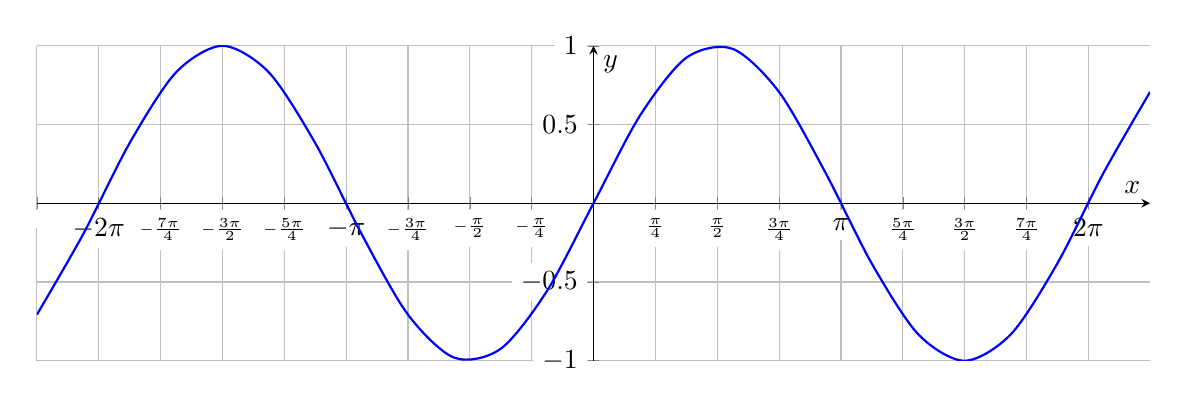
\begin{tikzpicture}
  \begin{axis}
	[% 290 of manual
	  xtick={-7.0686,-6.2831,...,7.0686},
	  xticklabels={% ref:http://tex.stackexchange.com/a/34958/ by Peter Grill
		,
		{$-2\pi$},
		{\tiny$-\frac{7\pi}{4}$},
		{\tiny$-\frac{3\pi}{2}$},
		{\tiny$-\frac{5\pi}{4}$},
		{$-\pi$},
		{\tiny$-\frac{3\pi}{4}$},
		{\tiny$-\frac{\pi}{2}$},
		{\tiny$-\frac{\pi}{4}$},
		{$0$},
		{\tiny$\frac{\pi}{4}$},
		{\tiny$\frac{\pi}{2}$},
		{\tiny$\frac{3\pi}{4}$},
		{$\pi$},
		{\tiny$\frac{5\pi}{4}$},
		{\tiny$\frac{3\pi}{2}$},
		{\tiny$\frac{7\pi}{4}$},
		{$2\pi$},
	  },
	  grid=major,
	  x=10mm,
	  y=20mm,
	  axis x line=center,% 218
	  axis y line=center,
	  xlabel={$x$},
	  ylabel={$y$},
	  every tick label/.style={fill=white},% 309
	]
  \addplot% ref: http://tex.stackexchange.com/a/147772/ by Harish Kumar
	[
	  domain=-2.25*pi:2.25*pi,
	  smooth,
	  blue,
	  thick,
	]
	plot {sin(deg(x))};
  \end{axis}
\end{tikzpicture}
\end{document}
